\documentclass{standalone}
\usepackage{tikz}
\usetikzlibrary{matrix, positioning, shapes.geometric, calc}

\begin{document}
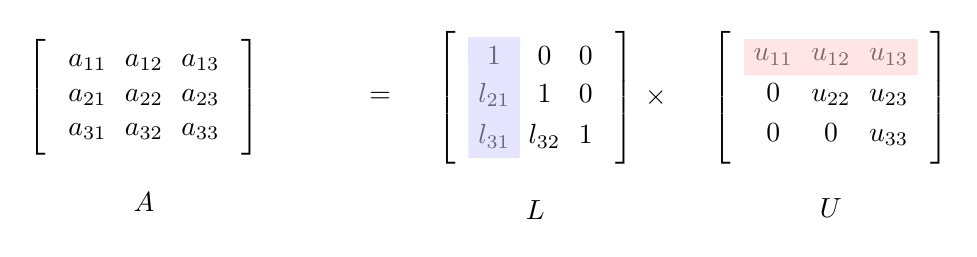
\begin{tikzpicture}
    % Matrix A
    \matrix (A) [matrix of math nodes, left delimiter={[}, right delimiter={]}] {
            a_{11} & a_{12} & a_{13} \\
            a_{21} & a_{22} & a_{23} \\
            a_{31} & a_{32} & a_{33} \\
        };

    \node at (A.south) [below=0.3cm] {$A$};

    % Equals sign
    \node at (3,0) {$=$};

    % Matrix L
    \matrix (L) [matrix of math nodes, left delimiter={[}, right delimiter={]}, anchor=west] at (4,0) {
            \ 1 \ & 0 & 0 \\
            l_{21} & 1 & 0 \\
            l_{31} & l_{32} & 1 \\
        };

    \node at (L.south) [below=0.3cm] {$L$};

    % Times sign
    \node at (6.5,0) {$\times$};

    % Matrix U
    \matrix (U) [matrix of math nodes, left delimiter={[}, right delimiter={]}, anchor=west] at (7.5,0) {
            u_{11} & u_{12} & u_{13} \\
            0 & u_{22} & u_{23} \\
            0 & 0 & u_{33} \\
        };

    \node at (U.south) [below=0.3cm] {$U$};

    % Color coding
    \fill[blue!20, opacity=0.5] (L-1-1.north west) -- (L-1-1.north east) -- (L-3-1.south east) -- (L-3-1.south west) -- cycle;
    \fill[red!20, opacity=0.5] (U-1-1.north west) -- (U-1-3.north east) -- (U-1-3.south east) -- (U-1-1.south west) -- cycle;
\end{tikzpicture}
\end{document}
